%!Tex Root = ../main.tex
% ./Packete.tex
% ./Design.tex
% ./Deklarationen.tex
% ./Vorbereitung.tex
% ./Aufgabe1.tex
% ./Aufgabe3.tex
% ./Aufgabe4.tex
% ./Appendix.tex

\section{Aufgabe 2}

\setcounter{exercise}{1}

\begin{frame}{Aufgabe \thesection}{n-Bit Inkrementer $INC_n$}
  \begin{solutionnoinc}
    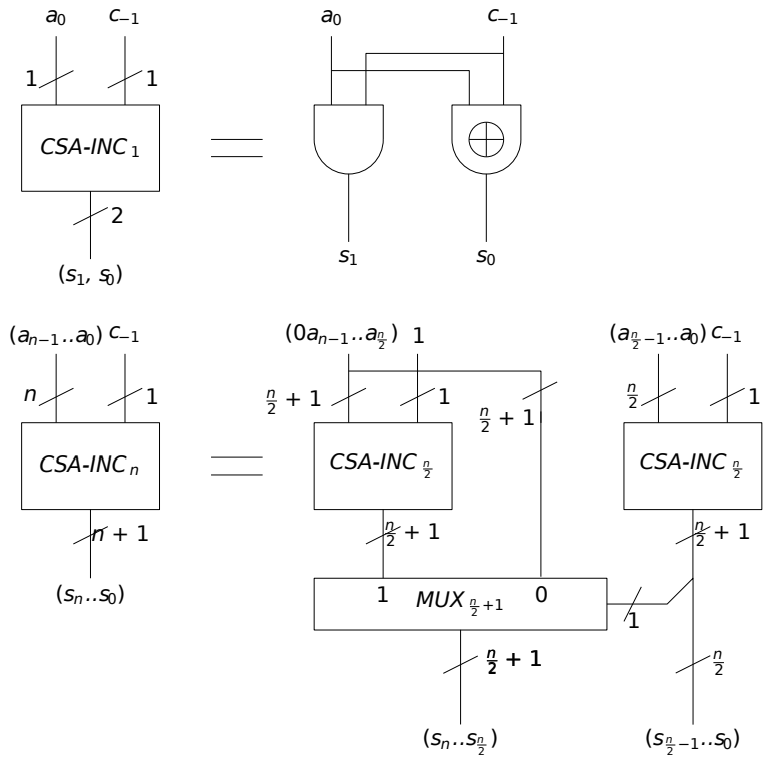
\includegraphics[height=0.6\paperheight, center]{figures/incrementer.png}
  \end{solutionnoinc}
\end{frame} 

\begin{frame}{Aufgabe \thesection}{n-Bit Inkrementer $INC_n$}
  \begin{solution}
    \centering
    % Important: If latex complains about unicode characters,
% please use "\usepackage[utf8x]{inputenc}" in your preamble
% You can change the size of the picture by putting it into the construct:
% 1) \resizebox{10cm}{!}{"below picture"} to scale horizontally to 10 cm
\resizebox{!}{6cm}{%"below picture"} to scale vertically to 15 cm
% 3) \resizebox{10cm}{15cm}{"below picture"} a combination of above two
% It is not recomended to use the scale option of the tikzpicture environment.
% https://tex.stackexchange.com/questions/438466/how-may-i-rotate-a-tikzpicture
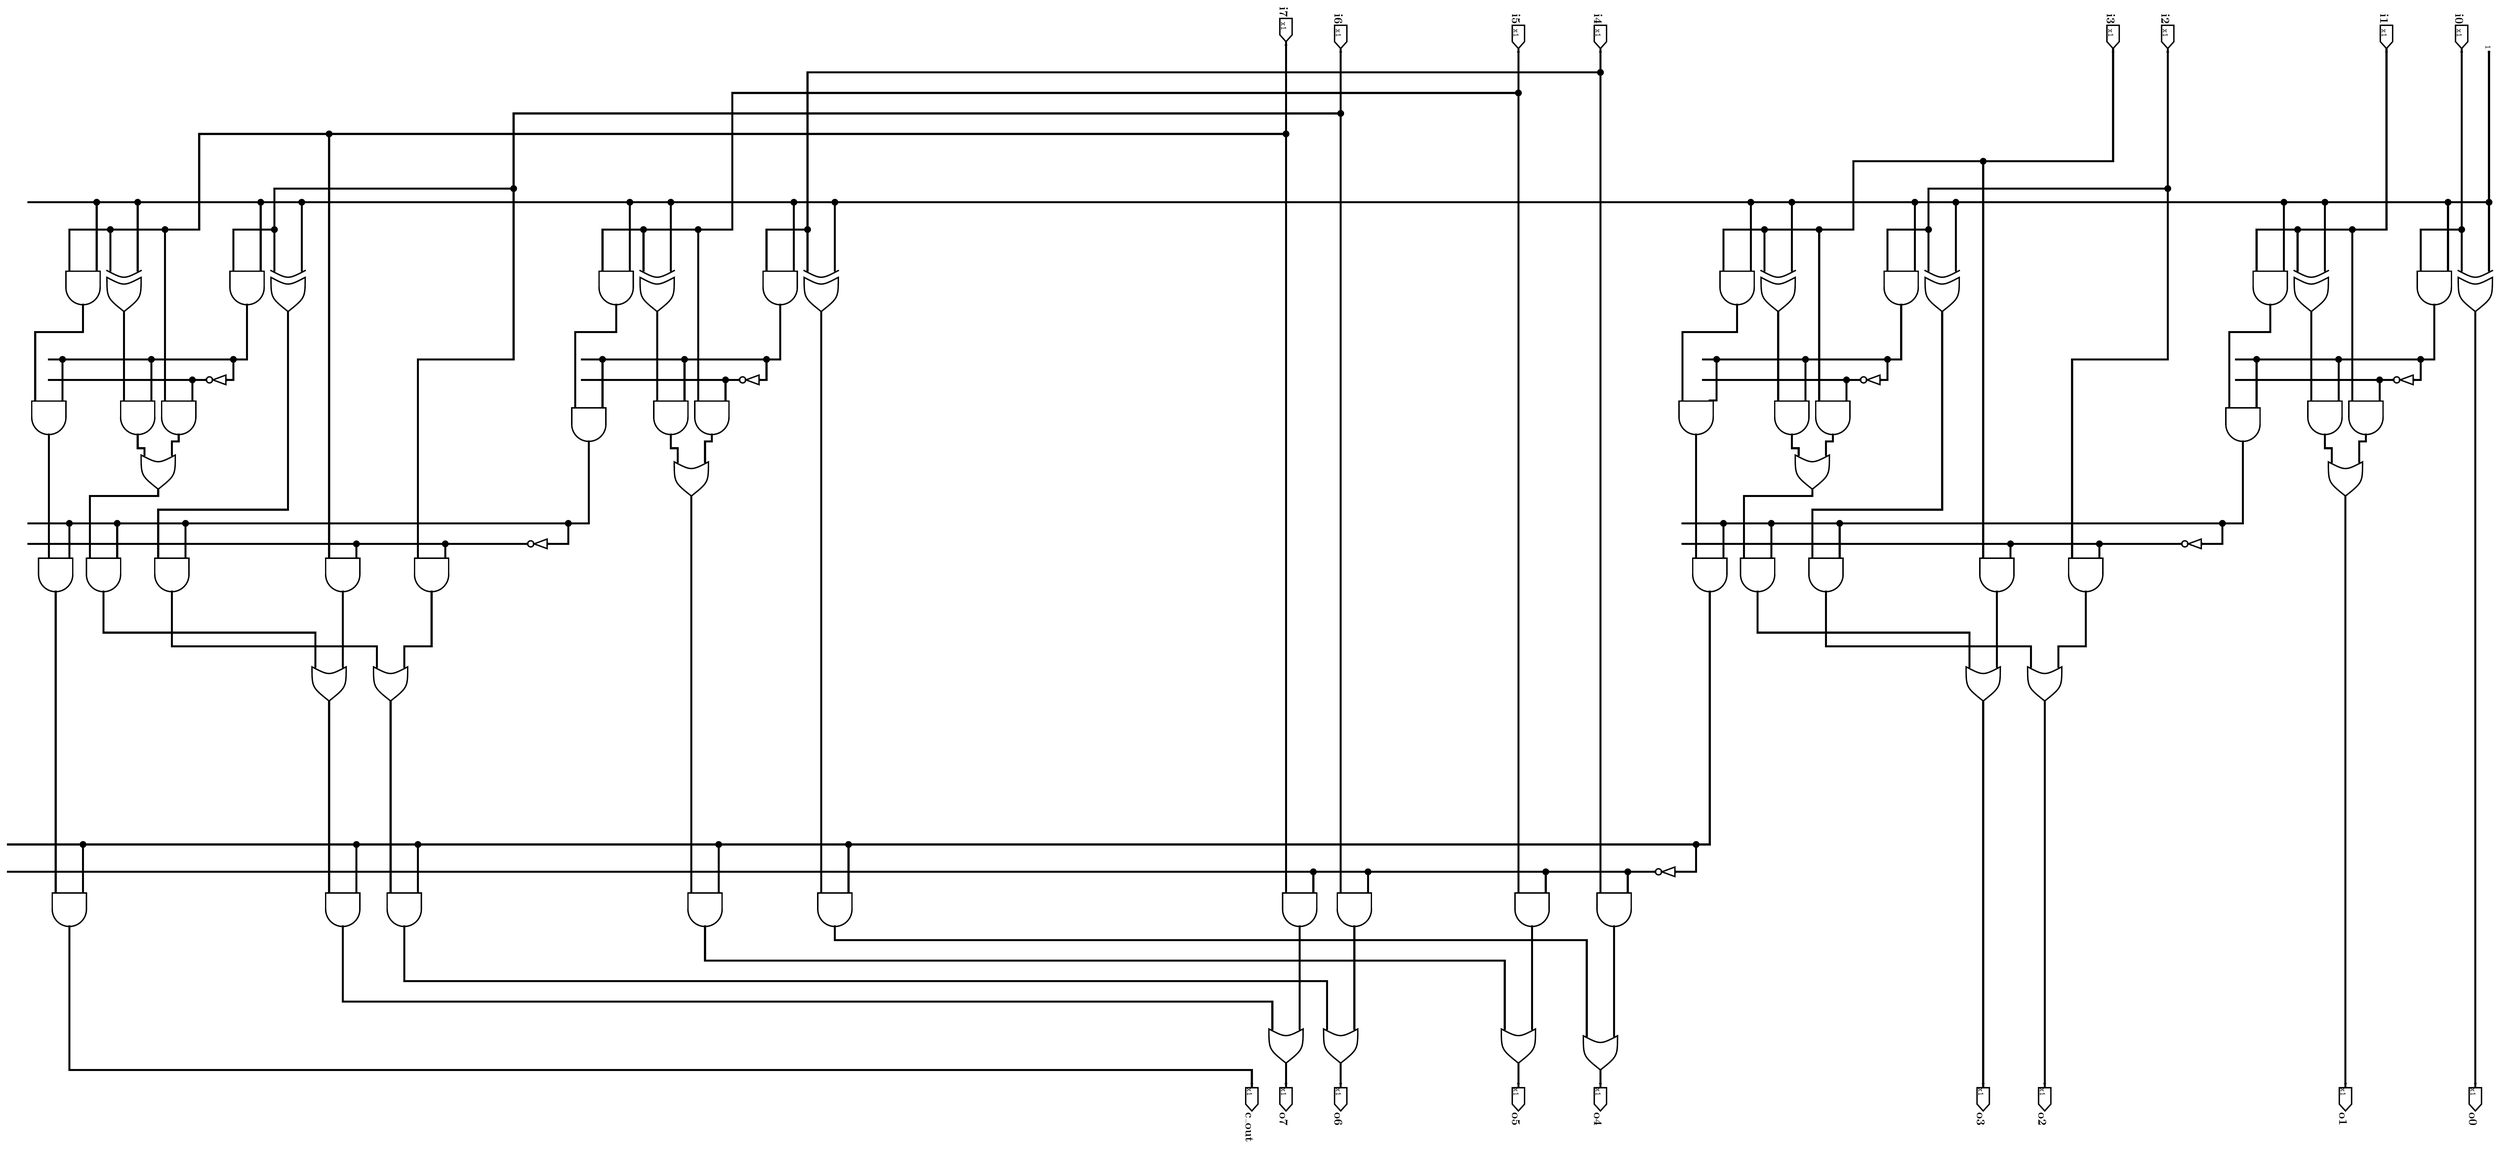
\begin{tikzpicture}[x=1pt,y=-1pt,line cap=rect,rotate=270,transform shape]
\def\logisimfontA#1{\fontfamily{cmr}{#1}} % Replaced by logisim, original font was "SansSerif"
\def\logisimfontB#1{\fontfamily{cmtt}{#1}} % Replaced by logisim, original font was "Monospaced"
\definecolor{custcol_0_0_0}{RGB}{0, 0, 0}
\definecolor{custcol_ff_ff_ff}{RGB}{255, 255, 255}
\draw [line width=3.0pt, custcol_0_0_0 ]  (1021.0,663.0) -- (1581.0,663.0) ;
\draw [line width=3.0pt, custcol_0_0_0 ]  (451.0,2453.0) -- (1301.0,2453.0) ;
\draw [line width=3.0pt, custcol_0_0_0 ]  (811.0,3553.0) -- (761.0,3553.0) -- (761.0,3613.0) ;
\draw [line width=3.0pt, custcol_0_0_0 ]  (521.0,383.0) -- (521.0,353.0) -- (591.0,353.0) ;
\draw [line width=3.0pt, custcol_0_0_0 ]  (1561.0,1313.0) -- (1581.0,1313.0) ;
\draw [line width=3.0pt, custcol_0_0_0 ]  (451.0,273.0) -- (581.0,273.0) ;
\draw [line width=3.0pt, custcol_0_0_0 ]  (1271.0,3643.0) -- (1271.0,1733.0) -- (1301.0,1733.0) ;
\draw [line width=3.0pt, custcol_0_0_0 ]  (451.0,3473.0) -- (581.0,3473.0) ;
\draw [line width=3.0pt, custcol_0_0_0 ]  (291.0,3453.0) -- (291.0,3513.0) -- (291.0,3613.0) ;
\draw [line width=3.0pt, custcol_0_0_0 ]  (1551.0,1693.0) -- (1581.0,1693.0) ;
\draw [line width=3.0pt, custcol_0_0_0 ]  (1551.0,1773.0) -- (1581.0,1773.0) ;
\draw [line width=3.0pt, custcol_0_0_0 ]  (631.0,1173.0) -- (811.0,1173.0) ;
\draw [line width=3.0pt, custcol_0_0_0 ]  (641.0,373.0) -- (761.0,373.0) -- (761.0,403.0) -- (761.0,963.0) -- (811.0,963.0) ;
\draw [line width=3.0pt, custcol_0_0_0 ]  (1021.0,3083.0) -- (1301.0,3083.0) ;
\draw [line width=3.0pt, custcol_0_0_0 ]  (761.0,963.0) -- (761.0,1063.0) -- (811.0,1063.0) ;
\draw [line width=3.0pt, custcol_0_0_0 ]  (191.0,3173.0) -- (811.0,3173.0) ;
\draw [line width=3.0pt, custcol_0_0_0 ]  (551.0,933.0) -- (551.0,953.0) -- (551.0,1163.0) ;
\draw [line width=3.0pt, custcol_0_0_0 ]  (551.0,953.0) -- (581.0,953.0) ;
\draw [line width=3.0pt, custcol_0_0_0 ]  (721.0,223.0) -- (1581.0,223.0) ;
\draw [line width=3.0pt, custcol_0_0_0 ]  (521.0,2803.0) -- (521.0,2773.0) -- (591.0,2773.0) ;
\draw [line width=3.0pt, custcol_0_0_0 ]  (521.0,2533.0) -- (521.0,2653.0) -- (581.0,2653.0) ;
\draw [line width=3.0pt, custcol_0_0_0 ]  (791.0,2883.0) -- (791.0,3003.0) -- (791.0,3133.0) -- (811.0,3133.0) ;
\draw [line width=3.0pt, custcol_0_0_0 ]  (1271.0,1233.0) -- (1271.0,1273.0) -- (1301.0,1273.0) ;
\draw [line width=3.0pt, custcol_0_0_0 ]  (451.0,2693.0) -- (581.0,2693.0) ;
\draw [line width=3.0pt, custcol_0_0_0 ]  (291.0,2433.0) -- (291.0,2493.0) ;
\draw [line width=3.0pt, custcol_0_0_0 ]  (291.0,2673.0) -- (291.0,2733.0) ;
\draw [line width=3.0pt, custcol_0_0_0 ]  (331.0,213.0) -- (331.0,293.0) -- (331.0,353.0) -- (391.0,353.0) ;
\draw [line width=3.0pt, custcol_0_0_0 ]  (1301.0,1653.0) -- (1271.0,1653.0) -- (1271.0,1733.0) ;
\draw [line width=3.0pt, custcol_0_0_0 ]  (331.0,3413.0) -- (331.0,3493.0) -- (331.0,3553.0) -- (391.0,3553.0) ;
\draw [line width=3.0pt, custcol_0_0_0 ]  (641.0,2793.0) -- (761.0,2793.0) -- (761.0,2823.0) ;
\draw [line width=3.0pt, custcol_0_0_0 ]  (811.0,3383.0) -- (761.0,3383.0) -- (761.0,2823.0) -- (791.0,2823.0) -- (791.0,2853.0) ;
\draw [line width=3.0pt, custcol_0_0_0 ]  (331.0,2633.0) -- (331.0,2713.0) ;
\draw [line width=3.0pt, custcol_0_0_0 ]  (1271.0,1203.0) -- (1271.0,1173.0) -- (1231.0,1173.0) -- (1231.0,2413.0) -- (1301.0,2413.0) ;
\draw [line width=3.0pt, custcol_0_0_0 ]  (1301.0,3133.0) -- (1231.0,3133.0) -- (1231.0,3533.0) -- (1301.0,3533.0) ;
\draw [line width=3.0pt, custcol_0_0_0 ]  (191.0,1773.0) -- (1301.0,1773.0) ;
\draw [line width=3.0pt, custcol_0_0_0 ]  (1231.0,3533.0) -- (1231.0,3643.0) ;
\draw [line width=3.0pt, custcol_0_0_0 ]  (711.0,3423.0) -- (721.0,3423.0) -- (721.0,3523.0) -- (811.0,3523.0) ;
\draw [line width=3.0pt, custcol_0_0_0 ]  (861.0,1153.0) -- (1231.0,1153.0) -- (1231.0,1173.0) ;
\draw [line width=3.0pt, custcol_0_0_0 ]  (521.0,1163.0) -- (521.0,1143.0) -- (581.0,1143.0) -- (581.0,1153.0) ;
\draw [line width=3.0pt, custcol_0_0_0 ]  (761.0,3383.0) -- (761.0,3483.0) -- (811.0,3483.0) ;
\draw [line width=3.0pt, custcol_0_0_0 ]  (1021.0,753.0) -- (1581.0,753.0) ;
\draw [line width=3.0pt, custcol_0_0_0 ]  (161.0,1693.0) -- (161.0,2903.0) -- (271.0,2903.0) -- (521.0,2903.0) -- (521.0,3043.0) -- (811.0,3043.0) ;
\draw [line width=3.0pt, custcol_0_0_0 ]  (451.0,813.0) -- (741.0,813.0) -- (741.0,1003.0) -- (811.0,1003.0) ;
\draw [line width=3.0pt, custcol_0_0_0 ]  (441.0,3533.0) -- (481.0,3533.0) -- (481.0,3603.0) -- (581.0,3603.0) ;
\draw [line width=3.0pt, custcol_0_0_0 ]  (271.0,2903.0) -- (271.0,3253.0) -- (331.0,3253.0) -- (331.0,3313.0) -- (391.0,3313.0) ;
\draw [line width=3.0pt, custcol_0_0_0 ]  (861.0,3573.0) -- (1301.0,3573.0) ;
\draw [line width=3.0pt, custcol_0_0_0 ]  (441.0,333.0) -- (481.0,333.0) -- (481.0,393.0) -- (591.0,393.0) ;
\draw [line width=3.0pt, custcol_0_0_0 ]  (551.0,153.0) -- (551.0,173.0) -- (551.0,383.0) ;
\draw [line width=3.0pt, custcol_0_0_0 ]  (581.0,3563.0) -- (521.0,3563.0) -- (521.0,3583.0) ;
\draw [line width=3.0pt, custcol_0_0_0 ]  (551.0,3353.0) -- (551.0,3373.0) -- (551.0,3583.0) ;
\draw [line width=3.0pt, custcol_0_0_0 ]  (791.0,463.0) -- (791.0,583.0) -- (811.0,583.0) ;
\draw [line width=3.0pt, custcol_0_0_0 ]  (551.0,3373.0) -- (581.0,3373.0) ;
\draw [line width=3.0pt, custcol_0_0_0 ]  (131.0,1433.0) -- (1301.0,1433.0) ;
\draw [line width=3.0pt, custcol_0_0_0 ]  (1231.0,2413.0) -- (1231.0,2603.0) ;
\draw [line width=3.0pt, custcol_0_0_0 ]  (551.0,173.0) -- (581.0,173.0) ;
\draw [line width=3.0pt, custcol_0_0_0 ]  (521.0,233.0) -- (521.0,353.0) ;
\draw [line width=3.0pt, custcol_0_0_0 ]  (721.0,2643.0) -- (1301.0,2643.0) ;
\draw [line width=3.0pt, custcol_0_0_0 ]  (761.0,1063.0) -- (761.0,1133.0) -- (811.0,1133.0) ;
\draw [line width=3.0pt, custcol_0_0_0 ]  (521.0,3433.0) -- (521.0,3563.0) ;
\draw [line width=3.0pt, custcol_0_0_0 ]  (761.0,3483.0) -- (761.0,3553.0) ;
\draw [line width=3.0pt, custcol_0_0_0 ]  (791.0,583.0) -- (791.0,713.0) -- (791.0,1193.0) ;
\draw [line width=3.0pt, custcol_0_0_0 ]  (441.0,93.0) -- (521.0,93.0) -- (521.0,113.0) -- (521.0,233.0) -- (581.0,233.0) ;
\draw [line width=3.0pt, custcol_0_0_0 ]  (451.0,33.0) -- (1581.0,33.0) ;
\draw [line width=3.0pt, custcol_0_0_0 ]  (441.0,3293.0) -- (521.0,3293.0) -- (521.0,3313.0) -- (521.0,3433.0) -- (581.0,3433.0) ;
\draw [line width=3.0pt, custcol_0_0_0 ]  (791.0,713.0) -- (811.0,713.0) ;
\draw [line width=3.0pt, custcol_0_0_0 ]  (521.0,3313.0) -- (551.0,3313.0) -- (551.0,3323.0) ;
\draw [line width=3.0pt, custcol_0_0_0 ]  (711.0,1003.0) -- (721.0,1003.0) -- (721.0,1103.0) -- (811.0,1103.0) ;
\draw [line width=3.0pt, custcol_0_0_0 ]  (521.0,113.0) -- (551.0,113.0) -- (551.0,123.0) ;
\draw [line width=3.0pt, custcol_0_0_0 ]  (1271.0,1273.0) -- (1271.0,1393.0) -- (1271.0,1653.0) ;
\draw [line width=3.0pt, custcol_0_0_0 ]  (791.0,3133.0) -- (791.0,3613.0) ;
\draw [line width=3.0pt, custcol_0_0_0 ]  (761.0,1133.0) -- (761.0,1193.0) ;
\draw [line width=3.0pt, custcol_0_0_0 ]  (811.0,753.0) -- (231.0,753.0) -- (231.0,943.0) -- (331.0,943.0) -- (331.0,993.0) ;
\draw [line width=3.0pt, custcol_0_0_0 ]  (441.0,2513.0) -- (521.0,2513.0) -- (521.0,2533.0) -- (551.0,2533.0) -- (551.0,2543.0) ;
\draw [line width=3.0pt, custcol_0_0_0 ]  (1351.0,3553.0) -- (1561.0,3553.0) -- (1561.0,1823.0) -- (1581.0,1823.0) ;
\draw [line width=3.0pt, custcol_0_0_0 ]  (441.0,873.0) -- (521.0,873.0) -- (521.0,893.0) -- (551.0,893.0) -- (551.0,903.0) ;
\draw [line width=3.0pt, custcol_0_0_0 ]  (631.0,3583.0) -- (811.0,3583.0) ;
\draw [line width=3.0pt, custcol_0_0_0 ]  (271.0,483.0) -- (521.0,483.0) -- (521.0,623.0) -- (811.0,623.0) ;
\draw [line width=3.0pt, custcol_0_0_0 ]  (521.0,1143.0) -- (521.0,1013.0) -- (581.0,1013.0) ;
\draw [line width=3.0pt, custcol_0_0_0 ]  (1301.0,2603.0) -- (1231.0,2603.0) -- (1231.0,3043.0) -- (1231.0,3133.0) ;
\draw [line width=3.0pt, custcol_0_0_0 ]  (441.0,1113.0) -- (481.0,1113.0) -- (481.0,1193.0) -- (581.0,1193.0) ;
\draw [line width=3.0pt, custcol_0_0_0 ]  (331.0,2473.0) -- (101.0,2473.0) -- (101.0,1313.0) -- (1301.0,1313.0) ;
\draw [line width=3.0pt, custcol_0_0_0 ]  (451.0,3233.0) -- (741.0,3233.0) -- (741.0,3423.0) -- (811.0,3423.0) ;
\draw [line width=3.0pt, custcol_0_0_0 ]  (291.0,73.0) -- (391.0,73.0) ;
\draw [line width=3.0pt, custcol_0_0_0 ]  (291.0,313.0) -- (391.0,313.0) ;
\draw [line width=3.0pt, custcol_0_0_0 ]  (291.0,3273.0) -- (391.0,3273.0) ;
\draw [line width=3.0pt, custcol_0_0_0 ]  (291.0,3513.0) -- (391.0,3513.0) ;
\draw [line width=3.0pt, custcol_0_0_0 ]  (441.0,2753.0) -- (481.0,2753.0) -- (481.0,2813.0) -- (591.0,2813.0) ;
\draw [line width=3.0pt, custcol_0_0_0 ]  (551.0,2573.0) -- (551.0,2593.0) -- (551.0,2803.0) ;
\draw [line width=3.0pt, custcol_0_0_0 ]  (791.0,3003.0) -- (811.0,3003.0) ;
\draw [line width=3.0pt, custcol_0_0_0 ]  (551.0,2593.0) -- (581.0,2593.0) ;
\draw [line width=3.0pt, custcol_0_0_0 ]  (761.0,403.0) -- (791.0,403.0) -- (791.0,433.0) ;
\draw [line width=3.0pt, custcol_0_0_0 ]  (1231.0,3043.0) -- (1301.0,3043.0) ;
\draw [line width=3.0pt, custcol_0_0_0 ]  (521.0,893.0) -- (521.0,1013.0) ;
\draw [line width=3.0pt, custcol_0_0_0 ]  (521.0,2653.0) -- (521.0,2773.0) ;
\draw [line width=3.0pt, custcol_0_0_0 ]  (451.0,1053.0) -- (581.0,1053.0) ;
\draw [line width=3.0pt, custcol_0_0_0 ]  (1271.0,1393.0) -- (1301.0,1393.0) ;
\draw [line width=3.0pt, custcol_0_0_0 ]  (1021.0,3173.0) -- (1301.0,3173.0) ;
\draw [line width=3.0pt, custcol_0_0_0 ]  (291.0,1033.0) -- (291.0,1093.0) ;
\draw [line width=3.0pt, custcol_0_0_0 ]  (291.0,793.0) -- (291.0,853.0) ;
\draw [line width=3.0pt, custcol_0_0_0 ]  (331.0,1073.0) -- (331.0,1133.0) -- (391.0,1133.0) ;
\draw [line width=3.0pt, custcol_0_0_0 ]  (331.0,833.0) -- (331.0,893.0) -- (391.0,893.0) ;
\draw [line width=3.0pt, custcol_0_0_0 ]  (1551.0,1433.0) -- (1581.0,1433.0) ;
\fill [line width=3.0pt, custcol_0_0_0]  (161.0,1693.0) ellipse (5.0 and 5.0 );
\fill [line width=3.0pt, custcol_0_0_0]  (291.0,793.0) ellipse (5.0 and 5.0 );
\fill [line width=3.0pt, custcol_0_0_0]  (331.0,2633.0) ellipse (5.0 and 5.0 );
\fill [line width=3.0pt, custcol_0_0_0]  (551.0,953.0) ellipse (5.0 and 5.0 );
\fill [line width=3.0pt, custcol_0_0_0]  (1231.0,2413.0) ellipse (5.0 and 5.0 );
\fill [line width=3.0pt, custcol_0_0_0]  (291.0,853.0) ellipse (5.0 and 5.0 );
\fill [line width=3.0pt, custcol_0_0_0]  (791.0,713.0) ellipse (5.0 and 5.0 );
\fill [line width=3.0pt, custcol_0_0_0]  (521.0,893.0) ellipse (5.0 and 5.0 );
\fill [line width=3.0pt, custcol_0_0_0]  (331.0,2713.0) ellipse (5.0 and 5.0 );
\fill [line width=3.0pt, custcol_0_0_0]  (271.0,483.0) ellipse (5.0 and 5.0 );
\fill [line width=3.0pt, custcol_0_0_0]  (1231.0,3533.0) ellipse (5.0 and 5.0 );
\fill [line width=3.0pt, custcol_0_0_0]  (1271.0,1273.0) ellipse (5.0 and 5.0 );
\fill [line width=3.0pt, custcol_0_0_0]  (231.0,753.0) ellipse (5.0 and 5.0 );
\fill [line width=3.0pt, custcol_0_0_0]  (521.0,1013.0) ellipse (5.0 and 5.0 );
\fill [line width=3.0pt, custcol_0_0_0]  (761.0,2823.0) ellipse (5.0 and 5.0 );
\fill [line width=3.0pt, custcol_0_0_0]  (1231.0,2603.0) ellipse (5.0 and 5.0 );
\fill [line width=3.0pt, custcol_0_0_0]  (291.0,1033.0) ellipse (5.0 and 5.0 );
\fill [line width=3.0pt, custcol_0_0_0]  (291.0,13.0) ellipse (5.0 and 5.0 );
\fill [line width=3.0pt, custcol_0_0_0]  (331.0,833.0) ellipse (5.0 and 5.0 );
\fill [line width=3.0pt, custcol_0_0_0]  (1271.0,1393.0) ellipse (5.0 and 5.0 );
\fill [line width=3.0pt, custcol_0_0_0]  (551.0,173.0) ellipse (5.0 and 5.0 );
\fill [line width=3.0pt, custcol_0_0_0]  (291.0,1093.0) ellipse (5.0 and 5.0 );
\fill [line width=3.0pt, custcol_0_0_0]  (791.0,3003.0) ellipse (5.0 and 5.0 );
\fill [line width=3.0pt, custcol_0_0_0]  (191.0,3173.0) ellipse (5.0 and 5.0 );
\fill [line width=3.0pt, custcol_0_0_0]  (291.0,73.0) ellipse (5.0 and 5.0 );
\fill [line width=3.0pt, custcol_0_0_0]  (521.0,113.0) ellipse (5.0 and 5.0 );
\fill [line width=3.0pt, custcol_0_0_0]  (521.0,1143.0) ellipse (5.0 and 5.0 );
\fill [line width=3.0pt, custcol_0_0_0]  (291.0,3213.0) ellipse (5.0 and 5.0 );
\fill [line width=3.0pt, custcol_0_0_0]  (551.0,3373.0) ellipse (5.0 and 5.0 );
\fill [line width=3.0pt, custcol_0_0_0]  (761.0,963.0) ellipse (5.0 and 5.0 );
\fill [line width=3.0pt, custcol_0_0_0]  (331.0,993.0) ellipse (5.0 and 5.0 );
\fill [line width=3.0pt, custcol_0_0_0]  (521.0,233.0) ellipse (5.0 and 5.0 );
\fill [line width=3.0pt, custcol_0_0_0]  (291.0,3273.0) ellipse (5.0 and 5.0 );
\fill [line width=3.0pt, custcol_0_0_0]  (791.0,3133.0) ellipse (5.0 and 5.0 );
\fill [line width=3.0pt, custcol_0_0_0]  (521.0,3313.0) ellipse (5.0 and 5.0 );
\fill [line width=3.0pt, custcol_0_0_0]  (271.0,2903.0) ellipse (5.0 and 5.0 );
\fill [line width=3.0pt, custcol_0_0_0]  (291.0,253.0) ellipse (5.0 and 5.0 );
\fill [line width=3.0pt, custcol_0_0_0]  (331.0,1073.0) ellipse (5.0 and 5.0 );
\fill [line width=3.0pt, custcol_0_0_0]  (331.0,53.0) ellipse (5.0 and 5.0 );
\fill [line width=3.0pt, custcol_0_0_0]  (761.0,1063.0) ellipse (5.0 and 5.0 );
\fill [line width=3.0pt, custcol_0_0_0]  (1271.0,1653.0) ellipse (5.0 and 5.0 );
\fill [line width=3.0pt, custcol_0_0_0]  (291.0,313.0) ellipse (5.0 and 5.0 );
\fill [line width=3.0pt, custcol_0_0_0]  (521.0,353.0) ellipse (5.0 and 5.0 );
\fill [line width=3.0pt, custcol_0_0_0]  (521.0,3433.0) ellipse (5.0 and 5.0 );
\fill [line width=3.0pt, custcol_0_0_0]  (761.0,1133.0) ellipse (5.0 and 5.0 );
\fill [line width=3.0pt, custcol_0_0_0]  (1271.0,1733.0) ellipse (5.0 and 5.0 );
\fill [line width=3.0pt, custcol_0_0_0]  (291.0,3453.0) ellipse (5.0 and 5.0 );
\fill [line width=3.0pt, custcol_0_0_0]  (291.0,2433.0) ellipse (5.0 and 5.0 );
\fill [line width=3.0pt, custcol_0_0_0]  (331.0,3253.0) ellipse (5.0 and 5.0 );
\fill [line width=3.0pt, custcol_0_0_0]  (551.0,2593.0) ellipse (5.0 and 5.0 );
\fill [line width=3.0pt, custcol_0_0_0]  (331.0,213.0) ellipse (5.0 and 5.0 );
\fill [line width=3.0pt, custcol_0_0_0]  (1231.0,3043.0) ellipse (5.0 and 5.0 );
\fill [line width=3.0pt, custcol_0_0_0]  (291.0,3513.0) ellipse (5.0 and 5.0 );
\fill [line width=3.0pt, custcol_0_0_0]  (291.0,2493.0) ellipse (5.0 and 5.0 );
\fill [line width=3.0pt, custcol_0_0_0]  (521.0,2533.0) ellipse (5.0 and 5.0 );
\fill [line width=3.0pt, custcol_0_0_0]  (521.0,3563.0) ellipse (5.0 and 5.0 );
\fill [line width=3.0pt, custcol_0_0_0]  (331.0,293.0) ellipse (5.0 and 5.0 );
\fill [line width=3.0pt, custcol_0_0_0]  (1231.0,3133.0) ellipse (5.0 and 5.0 );
\fill [line width=3.0pt, custcol_0_0_0]  (101.0,1313.0) ellipse (5.0 and 5.0 );
\fill [line width=3.0pt, custcol_0_0_0]  (761.0,3383.0) ellipse (5.0 and 5.0 );
\fill [line width=3.0pt, custcol_0_0_0]  (331.0,3413.0) ellipse (5.0 and 5.0 );
\fill [line width=3.0pt, custcol_0_0_0]  (521.0,2653.0) ellipse (5.0 and 5.0 );
\fill [line width=3.0pt, custcol_0_0_0]  (131.0,1433.0) ellipse (5.0 and 5.0 );
\fill [line width=3.0pt, custcol_0_0_0]  (1231.0,1173.0) ellipse (5.0 and 5.0 );
\fill [line width=3.0pt, custcol_0_0_0]  (291.0,2673.0) ellipse (5.0 and 5.0 );
\fill [line width=3.0pt, custcol_0_0_0]  (331.0,3493.0) ellipse (5.0 and 5.0 );
\fill [line width=3.0pt, custcol_0_0_0]  (761.0,403.0) ellipse (5.0 and 5.0 );
\fill [line width=3.0pt, custcol_0_0_0]  (331.0,2473.0) ellipse (5.0 and 5.0 );
\fill [line width=3.0pt, custcol_0_0_0]  (761.0,3483.0) ellipse (5.0 and 5.0 );
\fill [line width=3.0pt, custcol_0_0_0]  (291.0,2733.0) ellipse (5.0 and 5.0 );
\fill [line width=3.0pt, custcol_0_0_0]  (521.0,2773.0) ellipse (5.0 and 5.0 );
\fill [line width=3.0pt, custcol_0_0_0]  (761.0,3553.0) ellipse (5.0 and 5.0 );
\fill [line width=3.0pt, custcol_0_0_0]  (191.0,1773.0) ellipse (5.0 and 5.0 );
\fill [line width=3.0pt, custcol_0_0_0]  (791.0,583.0) ellipse (5.0 and 5.0 );
\draw [line width=3.0pt, custcol_0_0_0 ]  (56.0,1773.0) -- (61.0,1773.0) -- (191.0,1773.0) -- (191.0,3173.0) -- (191.0,3363.0) -- (331.0,3363.0) -- (331.0,3413.0) -- (581.0,3413.0) ;
\draw [line width=2.0pt, custcol_0_0_0 ]  (46.0,1782.0) -- (56.0,1773.0) -- (46.0,1764.0) -- (22.0,1764.0) -- (22.0,1782.0) -- cycle;
\logisimfontB{\fontsize{12pt}{12pt}\selectfont\node[inner sep=0, outer sep=0, custcol_0_0_0, anchor=base west] at  (27.0,1780.0)  {x1};}
\logisimfontA{\fontsize{16pt}{16pt}\fontseries{bx}\selectfont\node[inner sep=0, outer sep=0, custcol_0_0_0, anchor=base west] at  (5.0,1782.0)  {i7};}
\fill [line width=2.0pt, custcol_0_0_0]  (61.0,1773.0) ellipse (2.0 and 2.0 );
\draw [line width=3.0pt, custcol_0_0_0 ]  (66.0,1313.0) -- (71.0,1313.0) -- (101.0,1313.0) ;
\draw [line width=2.0pt, custcol_0_0_0 ]  (56.0,1322.0) -- (66.0,1313.0) -- (56.0,1304.0) -- (32.0,1304.0) -- (32.0,1322.0) -- cycle;
\logisimfontB{\fontsize{12pt}{12pt}\selectfont\node[inner sep=0, outer sep=0, custcol_0_0_0, anchor=base west] at  (37.0,1320.0)  {x1};}
\logisimfontA{\fontsize{16pt}{16pt}\fontseries{bx}\selectfont\node[inner sep=0, outer sep=0, custcol_0_0_0, anchor=base west] at  (15.0,1322.0)  {i4};}
\fill [line width=2.0pt, custcol_0_0_0]  (71.0,1313.0) ellipse (2.0 and 2.0 );
\draw [line width=3.0pt, custcol_0_0_0 ]  (66.0,1433.0) -- (71.0,1433.0) -- (131.0,1433.0) -- (131.0,2583.0) -- (331.0,2583.0) -- (331.0,2633.0) -- (581.0,2633.0) ;
\draw [line width=2.0pt, custcol_0_0_0 ]  (56.0,1442.0) -- (66.0,1433.0) -- (56.0,1424.0) -- (32.0,1424.0) -- (32.0,1442.0) -- cycle;
\logisimfontB{\fontsize{12pt}{12pt}\selectfont\node[inner sep=0, outer sep=0, custcol_0_0_0, anchor=base west] at  (37.0,1440.0)  {x1};}
\logisimfontA{\fontsize{16pt}{16pt}\fontseries{bx}\selectfont\node[inner sep=0, outer sep=0, custcol_0_0_0, anchor=base west] at  (15.0,1442.0)  {i5};}
\fill [line width=2.0pt, custcol_0_0_0]  (71.0,1433.0) ellipse (2.0 and 2.0 );
\draw [line width=3.0pt, custcol_0_0_0 ]  (66.0,1693.0) -- (71.0,1693.0) -- (161.0,1693.0) -- (1301.0,1693.0) ;
\draw [line width=2.0pt, custcol_0_0_0 ]  (56.0,1702.0) -- (66.0,1693.0) -- (56.0,1684.0) -- (32.0,1684.0) -- (32.0,1702.0) -- cycle;
\logisimfontB{\fontsize{12pt}{12pt}\selectfont\node[inner sep=0, outer sep=0, custcol_0_0_0, anchor=base west] at  (37.0,1700.0)  {x1};}
\logisimfontA{\fontsize{16pt}{16pt}\fontseries{bx}\selectfont\node[inner sep=0, outer sep=0, custcol_0_0_0, anchor=base west] at  (15.0,1702.0)  {i6};}
\fill [line width=2.0pt, custcol_0_0_0]  (71.0,1693.0) ellipse (2.0 and 2.0 );
\draw [line width=3.0pt, custcol_0_0_0 ]  (1585.0,33.0) -- (1582.0,33.0) ;
\draw [line width=2.0pt, custcol_0_0_0 ]  (1611.0,24.0) -- (1621.0,33.0) -- (1611.0,42.0) -- (1587.0,42.0) -- (1587.0,24.0) -- cycle;
\logisimfontB{\fontsize{12pt}{12pt}\selectfont\node[inner sep=0, outer sep=0, custcol_0_0_0, anchor=base west] at  (1587.0,40.0)  {x1};}
\logisimfontA{\fontsize{16pt}{16pt}\fontseries{bx}\selectfont\node[inner sep=0, outer sep=0, custcol_0_0_0, anchor=base west] at  (1623.0,42.0)  {o0};}
\fill [line width=2.0pt, custcol_0_0_0]  (1581.0,33.0) ellipse (2.0 and 2.0 );
\draw [line width=3.0pt, custcol_0_0_0 ]  (1585.0,223.0) -- (1582.0,223.0) ;
\draw [line width=2.0pt, custcol_0_0_0 ]  (1611.0,214.0) -- (1621.0,223.0) -- (1611.0,232.0) -- (1587.0,232.0) -- (1587.0,214.0) -- cycle;
\logisimfontB{\fontsize{12pt}{12pt}\selectfont\node[inner sep=0, outer sep=0, custcol_0_0_0, anchor=base west] at  (1587.0,230.0)  {x1};}
\logisimfontA{\fontsize{16pt}{16pt}\fontseries{bx}\selectfont\node[inner sep=0, outer sep=0, custcol_0_0_0, anchor=base west] at  (1623.0,232.0)  {o1};}
\fill [line width=2.0pt, custcol_0_0_0]  (1581.0,223.0) ellipse (2.0 and 2.0 );
\draw [line width=3.0pt, custcol_0_0_0 ]  (861.0,3023.0) -- (941.0,3023.0) -- (941.0,3063.0) -- (971.0,3063.0) -- (971.0,3063.0) ;
\draw [line width=3.0pt, custcol_0_0_0 ]  (861.0,3403.0) -- (941.0,3403.0) -- (941.0,3103.0) -- (971.0,3103.0) -- (971.0,3103.0) ;
\draw [line width=2.0pt, custcol_0_0_0 ]  (1021.0,3083.0) .. controls  (1001.0,3058.0)  ..  (971.0,3058.0) .. controls  (984.0,3083.0)  ..  (971.0,3108.0) .. controls  (1001.0,3108.0)  ..  (1021.0,3083.0) -- cycle ;
\draw [line width=3.0pt, custcol_0_0_0 ]  (861.0,3153.0) -- (971.0,3153.0) -- (971.0,3153.0) ;
\draw [line width=3.0pt, custcol_0_0_0 ]  (861.0,3503.0) -- (921.0,3503.0) -- (921.0,3193.0) -- (971.0,3193.0) -- (971.0,3193.0) ;
\draw [line width=2.0pt, custcol_0_0_0 ]  (1021.0,3173.0) .. controls  (1001.0,3148.0)  ..  (971.0,3148.0) .. controls  (984.0,3173.0)  ..  (971.0,3198.0) .. controls  (1001.0,3198.0)  ..  (1021.0,3173.0) -- cycle ;
\draw [line width=3.0pt, custcol_0_0_0 ]  (861.0,603.0) -- (941.0,603.0) -- (941.0,643.0) -- (971.0,643.0) -- (971.0,643.0) ;
\draw [line width=3.0pt, custcol_0_0_0 ]  (861.0,983.0) -- (941.0,983.0) -- (941.0,683.0) -- (971.0,683.0) -- (971.0,683.0) ;
\draw [line width=2.0pt, custcol_0_0_0 ]  (1021.0,663.0) .. controls  (1001.0,638.0)  ..  (971.0,638.0) .. controls  (984.0,663.0)  ..  (971.0,688.0) .. controls  (1001.0,688.0)  ..  (1021.0,663.0) -- cycle ;
\draw [line width=3.0pt, custcol_0_0_0 ]  (861.0,733.0) -- (971.0,733.0) -- (971.0,733.0) ;
\draw [line width=3.0pt, custcol_0_0_0 ]  (971.0,773.0) -- (971.0,773.0) -- (921.0,773.0) -- (921.0,1083.0) -- (861.0,1083.0) ;
\draw [line width=2.0pt, custcol_0_0_0 ]  (1021.0,753.0) .. controls  (1001.0,728.0)  ..  (971.0,728.0) .. controls  (984.0,753.0)  ..  (971.0,778.0) .. controls  (1001.0,778.0)  ..  (1021.0,753.0) -- cycle ;
\draw [line width=2.0pt, custcol_0_0_0 ]  (1271.0,1223.0) -- (1278.0,1204.0) -- (1264.0,1204.0) -- cycle;
\draw [line width=2.0pt, custcol_0_0_0, rotate around={-270: (1271.0,1228.0) }]  (1271.0,1228.0) ellipse (4.5 and 4.5 );
\fill [line width=2.0pt, custcol_0_0_0]  (1271.0,1233.0) ellipse (2.0 and 2.0 );
\fill [line width=2.0pt, custcol_0_0_0]  (1271.0,1203.0) ellipse (2.0 and 2.0 );
\draw [line width=2.0pt, custcol_0_0_0] (1326.0,1318.0) arc (90.0:-90.0:25.0 and 25.0 );
\draw [line width=2.0pt, custcol_0_0_0 ]  (1326.0,1268.0) -- (1302.0,1268.0) -- (1302.0,1318.0) -- (1326.0,1318.0) ;
\draw [line width=2.0pt, custcol_0_0_0] (1326.0,1438.0) arc (90.0:-90.0:25.0 and 25.0 );
\draw [line width=2.0pt, custcol_0_0_0 ]  (1326.0,1388.0) -- (1302.0,1388.0) -- (1302.0,1438.0) -- (1326.0,1438.0) ;
\draw [line width=2.0pt, custcol_0_0_0] (1326.0,1698.0) arc (90.0:-90.0:25.0 and 25.0 );
\draw [line width=2.0pt, custcol_0_0_0 ]  (1326.0,1648.0) -- (1302.0,1648.0) -- (1302.0,1698.0) -- (1326.0,1698.0) ;
\draw [line width=2.0pt, custcol_0_0_0] (1326.0,1778.0) arc (90.0:-90.0:25.0 and 25.0 );
\draw [line width=2.0pt, custcol_0_0_0 ]  (1326.0,1728.0) -- (1302.0,1728.0) -- (1302.0,1778.0) -- (1326.0,1778.0) ;
\draw [line width=2.0pt, custcol_0_0_0] (1326.0,2458.0) arc (90.0:-90.0:25.0 and 25.0 );
\draw [line width=2.0pt, custcol_0_0_0 ]  (1326.0,2408.0) -- (1302.0,2408.0) -- (1302.0,2458.0) -- (1326.0,2458.0) ;
\draw [line width=2.0pt, custcol_0_0_0] (1326.0,2648.0) arc (90.0:-90.0:25.0 and 25.0 );
\draw [line width=2.0pt, custcol_0_0_0 ]  (1326.0,2598.0) -- (1302.0,2598.0) -- (1302.0,2648.0) -- (1326.0,2648.0) ;
\draw [line width=2.0pt, custcol_0_0_0] (1326.0,3088.0) arc (90.0:-90.0:25.0 and 25.0 );
\draw [line width=2.0pt, custcol_0_0_0 ]  (1326.0,3038.0) -- (1302.0,3038.0) -- (1302.0,3088.0) -- (1326.0,3088.0) ;
\draw [line width=2.0pt, custcol_0_0_0] (1326.0,3178.0) arc (90.0:-90.0:25.0 and 25.0 );
\draw [line width=2.0pt, custcol_0_0_0 ]  (1326.0,3128.0) -- (1302.0,3128.0) -- (1302.0,3178.0) -- (1326.0,3178.0) ;
\draw [line width=2.0pt, custcol_0_0_0] (1326.0,3578.0) arc (90.0:-90.0:25.0 and 25.0 );
\draw [line width=2.0pt, custcol_0_0_0 ]  (1326.0,3528.0) -- (1302.0,3528.0) -- (1302.0,3578.0) -- (1326.0,3578.0) ;
\draw [line width=3.0pt, custcol_0_0_0 ]  (1351.0,1413.0) -- (1501.0,1413.0) -- (1501.0,1413.0) ;
\draw [line width=3.0pt, custcol_0_0_0 ]  (1351.0,2623.0) -- (1401.0,2623.0) -- (1401.0,1453.0) -- (1501.0,1453.0) -- (1501.0,1453.0) ;
\draw [line width=2.0pt, custcol_0_0_0 ]  (1551.0,1433.0) .. controls  (1531.0,1408.0)  ..  (1501.0,1408.0) .. controls  (1514.0,1433.0)  ..  (1501.0,1458.0) .. controls  (1531.0,1458.0)  ..  (1551.0,1433.0) -- cycle ;
\draw [line width=3.0pt, custcol_0_0_0 ]  (1351.0,1673.0) -- (1501.0,1673.0) -- (1501.0,1673.0) ;
\draw [line width=3.0pt, custcol_0_0_0 ]  (1501.0,1713.0) -- (1501.0,1713.0) -- (1431.0,1713.0) -- (1431.0,3063.0) -- (1351.0,3063.0) ;
\draw [line width=2.0pt, custcol_0_0_0 ]  (1551.0,1693.0) .. controls  (1531.0,1668.0)  ..  (1501.0,1668.0) .. controls  (1514.0,1693.0)  ..  (1501.0,1718.0) .. controls  (1531.0,1718.0)  ..  (1551.0,1693.0) -- cycle ;
\draw [line width=3.0pt, custcol_0_0_0 ]  (1351.0,1753.0) -- (1501.0,1753.0) -- (1501.0,1753.0) ;
\draw [line width=3.0pt, custcol_0_0_0 ]  (1501.0,1793.0) -- (1501.0,1793.0) -- (1461.0,1793.0) -- (1461.0,3153.0) -- (1351.0,3153.0) ;
\draw [line width=2.0pt, custcol_0_0_0 ]  (1551.0,1773.0) .. controls  (1531.0,1748.0)  ..  (1501.0,1748.0) .. controls  (1514.0,1773.0)  ..  (1501.0,1798.0) .. controls  (1531.0,1798.0)  ..  (1551.0,1773.0) -- cycle ;
\draw [line width=3.0pt, custcol_0_0_0 ]  (1351.0,1293.0) -- (1511.0,1293.0) -- (1511.0,1293.0) ;
\draw [line width=3.0pt, custcol_0_0_0 ]  (1351.0,2433.0) -- (1371.0,2433.0) -- (1371.0,1333.0) -- (1511.0,1333.0) -- (1511.0,1333.0) ;
\draw [line width=2.0pt, custcol_0_0_0 ]  (1561.0,1313.0) .. controls  (1541.0,1288.0)  ..  (1511.0,1288.0) .. controls  (1524.0,1313.0)  ..  (1511.0,1338.0) .. controls  (1541.0,1338.0)  ..  (1561.0,1313.0) -- cycle ;
\draw [line width=2.0pt, custcol_0_0_0] (416.0,1138.0) arc (90.0:-90.0:25.0 and 25.0 );
\draw [line width=2.0pt, custcol_0_0_0 ]  (416.0,1088.0) -- (392.0,1088.0) -- (392.0,1138.0) -- (416.0,1138.0) ;
\draw [line width=2.0pt, custcol_0_0_0] (416.0,118.0) arc (90.0:-90.0:25.0 and 25.0 );
\draw [line width=2.0pt, custcol_0_0_0 ]  (416.0,68.0) -- (392.0,68.0) -- (392.0,118.0) -- (416.0,118.0) ;
\draw [line width=2.0pt, custcol_0_0_0] (416.0,2538.0) arc (90.0:-90.0:25.0 and 25.0 );
\draw [line width=2.0pt, custcol_0_0_0 ]  (416.0,2488.0) -- (392.0,2488.0) -- (392.0,2538.0) -- (416.0,2538.0) ;
\draw [line width=2.0pt, custcol_0_0_0] (416.0,2778.0) arc (90.0:-90.0:25.0 and 25.0 );
\draw [line width=2.0pt, custcol_0_0_0 ]  (416.0,2728.0) -- (392.0,2728.0) -- (392.0,2778.0) -- (416.0,2778.0) ;
\draw [line width=2.0pt, custcol_0_0_0] (416.0,3318.0) arc (90.0:-90.0:25.0 and 25.0 );
\draw [line width=2.0pt, custcol_0_0_0 ]  (416.0,3268.0) -- (392.0,3268.0) -- (392.0,3318.0) -- (416.0,3318.0) ;
\draw [line width=2.0pt, custcol_0_0_0] (416.0,3558.0) arc (90.0:-90.0:25.0 and 25.0 );
\draw [line width=2.0pt, custcol_0_0_0 ]  (416.0,3508.0) -- (392.0,3508.0) -- (392.0,3558.0) -- (416.0,3558.0) ;
\draw [line width=2.0pt, custcol_0_0_0] (416.0,358.0) arc (90.0:-90.0:25.0 and 25.0 );
\draw [line width=2.0pt, custcol_0_0_0 ]  (416.0,308.0) -- (392.0,308.0) -- (392.0,358.0) -- (416.0,358.0) ;
\draw [line width=2.0pt, custcol_0_0_0] (416.0,898.0) arc (90.0:-90.0:25.0 and 25.0 );
\draw [line width=2.0pt, custcol_0_0_0 ]  (416.0,848.0) -- (392.0,848.0) -- (392.0,898.0) -- (416.0,898.0) ;
\draw [line width=3.0pt, custcol_0_0_0 ]  (391.0,853.0) -- (291.0,853.0) -- (291.0,1033.0) -- (391.0,1033.0) -- (391.0,1033.0) ;
\draw [line width=3.0pt, custcol_0_0_0 ]  (581.0,993.0) -- (331.0,993.0) -- (331.0,1073.0) -- (391.0,1073.0) -- (391.0,1073.0) ;
\draw [line width=2.0pt, custcol_0_0_0 ]  (451.0,1053.0) .. controls  (431.0,1028.0)  ..  (401.0,1028.0) .. controls  (414.0,1053.0)  ..  (401.0,1078.0) .. controls  (431.0,1078.0)  ..  (451.0,1053.0) -- cycle ;
\draw [line width=2.0pt, custcol_0_0_0 ]  (391.0,1028.0) .. controls  (404.0,1053.0)  ..  (391.0,1078.0) ;
\draw [line width=3.0pt, custcol_0_0_0 ]  (71.0,13.0) -- (291.0,13.0) -- (391.0,13.0) -- (391.0,13.0) ;
\draw [line width=3.0pt, custcol_0_0_0 ]  (331.0,53.0) -- (391.0,53.0) -- (391.0,53.0) ;
\draw [line width=2.0pt, custcol_0_0_0 ]  (451.0,33.0) .. controls  (431.0,8.0)  ..  (401.0,8.0) .. controls  (414.0,33.0)  ..  (401.0,58.0) .. controls  (431.0,58.0)  ..  (451.0,33.0) -- cycle ;
\draw [line width=2.0pt, custcol_0_0_0 ]  (391.0,8.0) .. controls  (404.0,33.0)  ..  (391.0,58.0) ;
\draw [line width=3.0pt, custcol_0_0_0 ]  (391.0,2433.0) -- (391.0,2433.0) -- (291.0,2433.0) -- (291.0,1093.0) -- (391.0,1093.0) ;
\draw [line width=3.0pt, custcol_0_0_0 ]  (391.0,2473.0) -- (391.0,2473.0) -- (331.0,2473.0) -- (331.0,2533.0) -- (391.0,2533.0) ;
\draw [line width=2.0pt, custcol_0_0_0 ]  (451.0,2453.0) .. controls  (431.0,2428.0)  ..  (401.0,2428.0) .. controls  (414.0,2453.0)  ..  (401.0,2478.0) .. controls  (431.0,2478.0)  ..  (451.0,2453.0) -- cycle ;
\draw [line width=2.0pt, custcol_0_0_0 ]  (391.0,2428.0) .. controls  (404.0,2453.0)  ..  (391.0,2478.0) ;
\draw [line width=3.0pt, custcol_0_0_0 ]  (391.0,2493.0) -- (291.0,2493.0) -- (291.0,2673.0) -- (391.0,2673.0) -- (391.0,2673.0) ;
\draw [line width=3.0pt, custcol_0_0_0 ]  (391.0,2713.0) -- (391.0,2713.0) -- (331.0,2713.0) -- (331.0,2773.0) -- (391.0,2773.0) ;
\draw [line width=2.0pt, custcol_0_0_0 ]  (451.0,2693.0) .. controls  (431.0,2668.0)  ..  (401.0,2668.0) .. controls  (414.0,2693.0)  ..  (401.0,2718.0) .. controls  (431.0,2718.0)  ..  (451.0,2693.0) -- cycle ;
\draw [line width=2.0pt, custcol_0_0_0 ]  (391.0,2668.0) .. controls  (404.0,2693.0)  ..  (391.0,2718.0) ;
\draw [line width=3.0pt, custcol_0_0_0 ]  (391.0,2733.0) -- (291.0,2733.0) -- (291.0,3213.0) -- (391.0,3213.0) -- (391.0,3213.0) ;
\draw [line width=3.0pt, custcol_0_0_0 ]  (331.0,3253.0) -- (391.0,3253.0) -- (391.0,3253.0) ;
\draw [line width=2.0pt, custcol_0_0_0 ]  (451.0,3233.0) .. controls  (431.0,3208.0)  ..  (401.0,3208.0) .. controls  (414.0,3233.0)  ..  (401.0,3258.0) .. controls  (431.0,3258.0)  ..  (451.0,3233.0) -- cycle ;
\draw [line width=2.0pt, custcol_0_0_0 ]  (391.0,3208.0) .. controls  (404.0,3233.0)  ..  (391.0,3258.0) ;
\draw [line width=3.0pt, custcol_0_0_0 ]  (291.0,3213.0) -- (291.0,3273.0) -- (291.0,3453.0) -- (391.0,3453.0) -- (391.0,3453.0) ;
\draw [line width=3.0pt, custcol_0_0_0 ]  (331.0,3493.0) -- (391.0,3493.0) -- (391.0,3493.0) ;
\draw [line width=2.0pt, custcol_0_0_0 ]  (451.0,3473.0) .. controls  (431.0,3448.0)  ..  (401.0,3448.0) .. controls  (414.0,3473.0)  ..  (401.0,3498.0) .. controls  (431.0,3498.0)  ..  (451.0,3473.0) -- cycle ;
\draw [line width=2.0pt, custcol_0_0_0 ]  (391.0,3448.0) .. controls  (404.0,3473.0)  ..  (391.0,3498.0) ;
\draw [line width=3.0pt, custcol_0_0_0 ]  (291.0,13.0) -- (291.0,73.0) -- (291.0,253.0) -- (391.0,253.0) -- (391.0,253.0) ;
\draw [line width=3.0pt, custcol_0_0_0 ]  (331.0,293.0) -- (391.0,293.0) -- (391.0,293.0) ;
\draw [line width=2.0pt, custcol_0_0_0 ]  (451.0,273.0) .. controls  (431.0,248.0)  ..  (401.0,248.0) .. controls  (414.0,273.0)  ..  (401.0,298.0) .. controls  (431.0,298.0)  ..  (451.0,273.0) -- cycle ;
\draw [line width=2.0pt, custcol_0_0_0 ]  (391.0,248.0) .. controls  (404.0,273.0)  ..  (391.0,298.0) ;
\draw [line width=3.0pt, custcol_0_0_0 ]  (291.0,253.0) -- (291.0,313.0) -- (291.0,793.0) -- (391.0,793.0) -- (391.0,793.0) ;
\draw [line width=2.0pt, custcol_0_0_0 ]  (451.0,813.0) .. controls  (431.0,788.0)  ..  (401.0,788.0) .. controls  (414.0,813.0)  ..  (401.0,838.0) .. controls  (431.0,838.0)  ..  (451.0,813.0) -- cycle ;
\draw [line width=2.0pt, custcol_0_0_0 ]  (391.0,788.0) .. controls  (404.0,813.0)  ..  (391.0,838.0) ;
\draw [line width=2.0pt, custcol_0_0_0 ]  (551.0,923.0) -- (558.0,904.0) -- (544.0,904.0) -- cycle;
\draw [line width=2.0pt, custcol_0_0_0, rotate around={-270: (551.0,928.0) }]  (551.0,928.0) ellipse (4.5 and 4.5 );
\fill [line width=2.0pt, custcol_0_0_0]  (551.0,933.0) ellipse (2.0 and 2.0 );
\fill [line width=2.0pt, custcol_0_0_0]  (551.0,903.0) ellipse (2.0 and 2.0 );
\draw [line width=2.0pt, custcol_0_0_0 ]  (551.0,143.0) -- (558.0,124.0) -- (544.0,124.0) -- cycle;
\draw [line width=2.0pt, custcol_0_0_0, rotate around={-270: (551.0,148.0) }]  (551.0,148.0) ellipse (4.5 and 4.5 );
\fill [line width=2.0pt, custcol_0_0_0]  (551.0,153.0) ellipse (2.0 and 2.0 );
\fill [line width=2.0pt, custcol_0_0_0]  (551.0,123.0) ellipse (2.0 and 2.0 );
\draw [line width=2.0pt, custcol_0_0_0 ]  (551.0,2563.0) -- (558.0,2544.0) -- (544.0,2544.0) -- cycle;
\draw [line width=2.0pt, custcol_0_0_0, rotate around={-270: (551.0,2568.0) }]  (551.0,2568.0) ellipse (4.5 and 4.5 );
\fill [line width=2.0pt, custcol_0_0_0]  (551.0,2573.0) ellipse (2.0 and 2.0 );
\fill [line width=2.0pt, custcol_0_0_0]  (551.0,2543.0) ellipse (2.0 and 2.0 );
\draw [line width=2.0pt, custcol_0_0_0 ]  (551.0,3343.0) -- (558.0,3324.0) -- (544.0,3324.0) -- cycle;
\draw [line width=2.0pt, custcol_0_0_0, rotate around={-270: (551.0,3348.0) }]  (551.0,3348.0) ellipse (4.5 and 4.5 );
\fill [line width=2.0pt, custcol_0_0_0]  (551.0,3353.0) ellipse (2.0 and 2.0 );
\fill [line width=2.0pt, custcol_0_0_0]  (551.0,3323.0) ellipse (2.0 and 2.0 );
\draw [line width=2.0pt, custcol_0_0_0] (606.0,998.0) arc (90.0:-90.0:25.0 and 25.0 );
\draw [line width=2.0pt, custcol_0_0_0 ]  (606.0,948.0) -- (582.0,948.0) -- (582.0,998.0) -- (606.0,998.0) ;
\draw [line width=2.0pt, custcol_0_0_0] (606.0,1058.0) arc (90.0:-90.0:25.0 and 25.0 );
\draw [line width=2.0pt, custcol_0_0_0 ]  (606.0,1008.0) -- (582.0,1008.0) -- (582.0,1058.0) -- (606.0,1058.0) ;
\draw [line width=2.0pt, custcol_0_0_0] (606.0,1198.0) arc (90.0:-90.0:25.0 and 25.0 );
\draw [line width=2.0pt, custcol_0_0_0 ]  (606.0,1148.0) -- (582.0,1148.0) -- (582.0,1198.0) -- (606.0,1198.0) ;
\draw [line width=2.0pt, custcol_0_0_0] (606.0,2638.0) arc (90.0:-90.0:25.0 and 25.0 );
\draw [line width=2.0pt, custcol_0_0_0 ]  (606.0,2588.0) -- (582.0,2588.0) -- (582.0,2638.0) -- (606.0,2638.0) ;
\draw [line width=2.0pt, custcol_0_0_0] (606.0,2698.0) arc (90.0:-90.0:25.0 and 25.0 );
\draw [line width=2.0pt, custcol_0_0_0 ]  (606.0,2648.0) -- (582.0,2648.0) -- (582.0,2698.0) -- (606.0,2698.0) ;
\draw [line width=2.0pt, custcol_0_0_0] (606.0,218.0) arc (90.0:-90.0:25.0 and 25.0 );
\draw [line width=2.0pt, custcol_0_0_0 ]  (606.0,168.0) -- (582.0,168.0) -- (582.0,218.0) -- (606.0,218.0) ;
\draw [line width=2.0pt, custcol_0_0_0] (606.0,278.0) arc (90.0:-90.0:25.0 and 25.0 );
\draw [line width=2.0pt, custcol_0_0_0 ]  (606.0,228.0) -- (582.0,228.0) -- (582.0,278.0) -- (606.0,278.0) ;
\draw [line width=2.0pt, custcol_0_0_0] (606.0,3418.0) arc (90.0:-90.0:25.0 and 25.0 );
\draw [line width=2.0pt, custcol_0_0_0 ]  (606.0,3368.0) -- (582.0,3368.0) -- (582.0,3418.0) -- (606.0,3418.0) ;
\draw [line width=2.0pt, custcol_0_0_0] (606.0,3478.0) arc (90.0:-90.0:25.0 and 25.0 );
\draw [line width=2.0pt, custcol_0_0_0 ]  (606.0,3428.0) -- (582.0,3428.0) -- (582.0,3478.0) -- (606.0,3478.0) ;
\draw [line width=2.0pt, custcol_0_0_0] (606.0,3608.0) arc (90.0:-90.0:25.0 and 25.0 );
\draw [line width=2.0pt, custcol_0_0_0 ]  (606.0,3558.0) -- (582.0,3558.0) -- (582.0,3608.0) -- (606.0,3608.0) ;
\draw [line width=2.0pt, custcol_0_0_0] (616.0,2818.0) arc (90.0:-90.0:25.0 and 25.0 );
\draw [line width=2.0pt, custcol_0_0_0 ]  (616.0,2768.0) -- (592.0,2768.0) -- (592.0,2818.0) -- (616.0,2818.0) ;
\draw [line width=2.0pt, custcol_0_0_0] (616.0,398.0) arc (90.0:-90.0:25.0 and 25.0 );
\draw [line width=2.0pt, custcol_0_0_0 ]  (616.0,348.0) -- (592.0,348.0) -- (592.0,398.0) -- (616.0,398.0) ;
\draw [line width=3.0pt, custcol_0_0_0 ]  (631.0,973.0) -- (641.0,973.0) -- (641.0,983.0) -- (661.0,983.0) -- (661.0,983.0) ;
\draw [line width=3.0pt, custcol_0_0_0 ]  (631.0,1033.0) -- (651.0,1033.0) -- (651.0,1023.0) -- (661.0,1023.0) -- (661.0,1023.0) ;
\draw [line width=2.0pt, custcol_0_0_0 ]  (711.0,1003.0) .. controls  (691.0,978.0)  ..  (661.0,978.0) .. controls  (674.0,1003.0)  ..  (661.0,1028.0) .. controls  (691.0,1028.0)  ..  (711.0,1003.0) -- cycle ;
\draw [line width=3.0pt, custcol_0_0_0 ]  (631.0,3393.0) -- (641.0,3393.0) -- (641.0,3403.0) -- (661.0,3403.0) -- (661.0,3403.0) ;
\draw [line width=3.0pt, custcol_0_0_0 ]  (631.0,3453.0) -- (651.0,3453.0) -- (651.0,3443.0) -- (661.0,3443.0) -- (661.0,3443.0) ;
\draw [line width=2.0pt, custcol_0_0_0 ]  (711.0,3423.0) .. controls  (691.0,3398.0)  ..  (661.0,3398.0) .. controls  (674.0,3423.0)  ..  (661.0,3448.0) .. controls  (691.0,3448.0)  ..  (711.0,3423.0) -- cycle ;
\draw [line width=3.0pt, custcol_0_0_0 ]  (631.0,2613.0) -- (641.0,2613.0) -- (641.0,2623.0) -- (671.0,2623.0) -- (671.0,2623.0) ;
\draw [line width=3.0pt, custcol_0_0_0 ]  (631.0,2673.0) -- (651.0,2673.0) -- (651.0,2663.0) -- (671.0,2663.0) -- (671.0,2663.0) ;
\draw [line width=2.0pt, custcol_0_0_0 ]  (721.0,2643.0) .. controls  (701.0,2618.0)  ..  (671.0,2618.0) .. controls  (684.0,2643.0)  ..  (671.0,2668.0) .. controls  (701.0,2668.0)  ..  (721.0,2643.0) -- cycle ;
\draw [line width=3.0pt, custcol_0_0_0 ]  (631.0,193.0) -- (641.0,193.0) -- (641.0,203.0) -- (671.0,203.0) -- (671.0,203.0) ;
\draw [line width=3.0pt, custcol_0_0_0 ]  (631.0,253.0) -- (651.0,253.0) -- (651.0,243.0) -- (671.0,243.0) -- (671.0,243.0) ;
\draw [line width=2.0pt, custcol_0_0_0 ]  (721.0,223.0) .. controls  (701.0,198.0)  ..  (671.0,198.0) .. controls  (684.0,223.0)  ..  (671.0,248.0) .. controls  (701.0,248.0)  ..  (721.0,223.0) -- cycle ;
\draw [line width=2.0pt, custcol_0_0_0 ]  (791.0,2873.0) -- (798.0,2854.0) -- (784.0,2854.0) -- cycle;
\draw [line width=2.0pt, custcol_0_0_0, rotate around={-270: (791.0,2878.0) }]  (791.0,2878.0) ellipse (4.5 and 4.5 );
\fill [line width=2.0pt, custcol_0_0_0]  (791.0,2883.0) ellipse (2.0 and 2.0 );
\fill [line width=2.0pt, custcol_0_0_0]  (791.0,2853.0) ellipse (2.0 and 2.0 );
\draw [line width=2.0pt, custcol_0_0_0 ]  (791.0,453.0) -- (798.0,434.0) -- (784.0,434.0) -- cycle;
\draw [line width=2.0pt, custcol_0_0_0, rotate around={-270: (791.0,458.0) }]  (791.0,458.0) ellipse (4.5 and 4.5 );
\fill [line width=2.0pt, custcol_0_0_0]  (791.0,463.0) ellipse (2.0 and 2.0 );
\fill [line width=2.0pt, custcol_0_0_0]  (791.0,433.0) ellipse (2.0 and 2.0 );
\draw [line width=2.0pt, custcol_0_0_0] (836.0,1008.0) arc (90.0:-90.0:25.0 and 25.0 );
\draw [line width=2.0pt, custcol_0_0_0 ]  (836.0,958.0) -- (812.0,958.0) -- (812.0,1008.0) -- (836.0,1008.0) ;
\draw [line width=2.0pt, custcol_0_0_0] (836.0,1108.0) arc (90.0:-90.0:25.0 and 25.0 );
\draw [line width=2.0pt, custcol_0_0_0 ]  (836.0,1058.0) -- (812.0,1058.0) -- (812.0,1108.0) -- (836.0,1108.0) ;
\draw [line width=2.0pt, custcol_0_0_0] (836.0,1178.0) arc (90.0:-90.0:25.0 and 25.0 );
\draw [line width=2.0pt, custcol_0_0_0 ]  (836.0,1128.0) -- (812.0,1128.0) -- (812.0,1178.0) -- (836.0,1178.0) ;
\draw [line width=2.0pt, custcol_0_0_0] (836.0,3048.0) arc (90.0:-90.0:25.0 and 25.0 );
\draw [line width=2.0pt, custcol_0_0_0 ]  (836.0,2998.0) -- (812.0,2998.0) -- (812.0,3048.0) -- (836.0,3048.0) ;
\draw [line width=2.0pt, custcol_0_0_0] (836.0,3178.0) arc (90.0:-90.0:25.0 and 25.0 );
\draw [line width=2.0pt, custcol_0_0_0 ]  (836.0,3128.0) -- (812.0,3128.0) -- (812.0,3178.0) -- (836.0,3178.0) ;
\draw [line width=2.0pt, custcol_0_0_0] (836.0,3428.0) arc (90.0:-90.0:25.0 and 25.0 );
\draw [line width=2.0pt, custcol_0_0_0 ]  (836.0,3378.0) -- (812.0,3378.0) -- (812.0,3428.0) -- (836.0,3428.0) ;
\draw [line width=2.0pt, custcol_0_0_0] (836.0,3528.0) arc (90.0:-90.0:25.0 and 25.0 );
\draw [line width=2.0pt, custcol_0_0_0 ]  (836.0,3478.0) -- (812.0,3478.0) -- (812.0,3528.0) -- (836.0,3528.0) ;
\draw [line width=2.0pt, custcol_0_0_0] (836.0,3598.0) arc (90.0:-90.0:25.0 and 25.0 );
\draw [line width=2.0pt, custcol_0_0_0 ]  (836.0,3548.0) -- (812.0,3548.0) -- (812.0,3598.0) -- (836.0,3598.0) ;
\draw [line width=2.0pt, custcol_0_0_0] (836.0,628.0) arc (90.0:-90.0:25.0 and 25.0 );
\draw [line width=2.0pt, custcol_0_0_0 ]  (836.0,578.0) -- (812.0,578.0) -- (812.0,628.0) -- (836.0,628.0) ;
\draw [line width=2.0pt, custcol_0_0_0] (836.0,758.0) arc (90.0:-90.0:25.0 and 25.0 );
\draw [line width=2.0pt, custcol_0_0_0 ]  (836.0,708.0) -- (812.0,708.0) -- (812.0,758.0) -- (836.0,758.0) ;
\logisimfontB{\fontsize{12pt}{12pt}\selectfont\node[inner sep=0, outer sep=0, custcol_0_0_0, anchor=base west] at  (61.0,18.0)  {1};}
\fill [line width=1.0pt, custcol_0_0_0]  (71.0,13.0) ellipse (2.0 and 2.0 );
\draw [line width=3.0pt, custcol_0_0_0 ]  (66.0,483.0) -- (71.0,483.0) -- (271.0,483.0) -- (271.0,833.0) -- (331.0,833.0) -- (391.0,833.0) -- (391.0,833.0) ;
\draw [line width=2.0pt, custcol_0_0_0 ]  (56.0,492.0) -- (66.0,483.0) -- (56.0,474.0) -- (32.0,474.0) -- (32.0,492.0) -- cycle;
\logisimfontB{\fontsize{12pt}{12pt}\selectfont\node[inner sep=0, outer sep=0, custcol_0_0_0, anchor=base west] at  (37.0,490.0)  {x1};}
\logisimfontA{\fontsize{16pt}{16pt}\fontseries{bx}\selectfont\node[inner sep=0, outer sep=0, custcol_0_0_0, anchor=base west] at  (15.0,492.0)  {i2};}
\fill [line width=2.0pt, custcol_0_0_0]  (71.0,483.0) ellipse (2.0 and 2.0 );
\draw [line width=3.0pt, custcol_0_0_0 ]  (66.0,163.0) -- (71.0,163.0) -- (331.0,163.0) -- (331.0,213.0) -- (581.0,213.0) ;
\draw [line width=2.0pt, custcol_0_0_0 ]  (56.0,172.0) -- (66.0,163.0) -- (56.0,154.0) -- (32.0,154.0) -- (32.0,172.0) -- cycle;
\logisimfontB{\fontsize{12pt}{12pt}\selectfont\node[inner sep=0, outer sep=0, custcol_0_0_0, anchor=base west] at  (37.0,170.0)  {x1};}
\logisimfontA{\fontsize{16pt}{16pt}\fontseries{bx}\selectfont\node[inner sep=0, outer sep=0, custcol_0_0_0, anchor=base west] at  (15.0,172.0)  {i1};}
\fill [line width=2.0pt, custcol_0_0_0]  (71.0,163.0) ellipse (2.0 and 2.0 );
\draw [line width=3.0pt, custcol_0_0_0 ]  (66.0,563.0) -- (71.0,563.0) -- (231.0,563.0) -- (231.0,753.0) ;
\draw [line width=2.0pt, custcol_0_0_0 ]  (56.0,572.0) -- (66.0,563.0) -- (56.0,554.0) -- (32.0,554.0) -- (32.0,572.0) -- cycle;
\logisimfontB{\fontsize{12pt}{12pt}\selectfont\node[inner sep=0, outer sep=0, custcol_0_0_0, anchor=base west] at  (37.0,570.0)  {x1};}
\logisimfontA{\fontsize{16pt}{16pt}\fontseries{bx}\selectfont\node[inner sep=0, outer sep=0, custcol_0_0_0, anchor=base west] at  (15.0,572.0)  {i3};}
\fill [line width=2.0pt, custcol_0_0_0]  (71.0,563.0) ellipse (2.0 and 2.0 );
\draw [line width=3.0pt, custcol_0_0_0 ]  (1585.0,753.0) -- (1582.0,753.0) ;
\draw [line width=2.0pt, custcol_0_0_0 ]  (1611.0,744.0) -- (1621.0,753.0) -- (1611.0,762.0) -- (1587.0,762.0) -- (1587.0,744.0) -- cycle;
\logisimfontB{\fontsize{12pt}{12pt}\selectfont\node[inner sep=0, outer sep=0, custcol_0_0_0, anchor=base west] at  (1587.0,760.0)  {x1};}
\logisimfontA{\fontsize{16pt}{16pt}\fontseries{bx}\selectfont\node[inner sep=0, outer sep=0, custcol_0_0_0, anchor=base west] at  (1623.0,762.0)  {o3};}
\fill [line width=2.0pt, custcol_0_0_0]  (1581.0,753.0) ellipse (2.0 and 2.0 );
\draw [line width=3.0pt, custcol_0_0_0 ]  (1585.0,663.0) -- (1582.0,663.0) ;
\draw [line width=2.0pt, custcol_0_0_0 ]  (1611.0,654.0) -- (1621.0,663.0) -- (1611.0,672.0) -- (1587.0,672.0) -- (1587.0,654.0) -- cycle;
\logisimfontB{\fontsize{12pt}{12pt}\selectfont\node[inner sep=0, outer sep=0, custcol_0_0_0, anchor=base west] at  (1587.0,670.0)  {x1};}
\logisimfontA{\fontsize{16pt}{16pt}\fontseries{bx}\selectfont\node[inner sep=0, outer sep=0, custcol_0_0_0, anchor=base west] at  (1623.0,672.0)  {o2};}
\fill [line width=2.0pt, custcol_0_0_0]  (1581.0,663.0) ellipse (2.0 and 2.0 );
\draw [line width=3.0pt, custcol_0_0_0 ]  (1585.0,1433.0) -- (1582.0,1433.0) ;
\draw [line width=2.0pt, custcol_0_0_0 ]  (1611.0,1424.0) -- (1621.0,1433.0) -- (1611.0,1442.0) -- (1587.0,1442.0) -- (1587.0,1424.0) -- cycle;
\logisimfontB{\fontsize{12pt}{12pt}\selectfont\node[inner sep=0, outer sep=0, custcol_0_0_0, anchor=base west] at  (1587.0,1440.0)  {x1};}
\logisimfontA{\fontsize{16pt}{16pt}\fontseries{bx}\selectfont\node[inner sep=0, outer sep=0, custcol_0_0_0, anchor=base west] at  (1623.0,1442.0)  {o5};}
\fill [line width=2.0pt, custcol_0_0_0]  (1581.0,1433.0) ellipse (2.0 and 2.0 );
\draw [line width=3.0pt, custcol_0_0_0 ]  (1585.0,1313.0) -- (1582.0,1313.0) ;
\draw [line width=2.0pt, custcol_0_0_0 ]  (1611.0,1304.0) -- (1621.0,1313.0) -- (1611.0,1322.0) -- (1587.0,1322.0) -- (1587.0,1304.0) -- cycle;
\logisimfontB{\fontsize{12pt}{12pt}\selectfont\node[inner sep=0, outer sep=0, custcol_0_0_0, anchor=base west] at  (1587.0,1320.0)  {x1};}
\logisimfontA{\fontsize{16pt}{16pt}\fontseries{bx}\selectfont\node[inner sep=0, outer sep=0, custcol_0_0_0, anchor=base west] at  (1623.0,1322.0)  {o4};}
\fill [line width=2.0pt, custcol_0_0_0]  (1581.0,1313.0) ellipse (2.0 and 2.0 );
\draw [line width=3.0pt, custcol_0_0_0 ]  (1585.0,1693.0) -- (1582.0,1693.0) ;
\draw [line width=2.0pt, custcol_0_0_0 ]  (1611.0,1684.0) -- (1621.0,1693.0) -- (1611.0,1702.0) -- (1587.0,1702.0) -- (1587.0,1684.0) -- cycle;
\logisimfontB{\fontsize{12pt}{12pt}\selectfont\node[inner sep=0, outer sep=0, custcol_0_0_0, anchor=base west] at  (1587.0,1700.0)  {x1};}
\logisimfontA{\fontsize{16pt}{16pt}\fontseries{bx}\selectfont\node[inner sep=0, outer sep=0, custcol_0_0_0, anchor=base west] at  (1623.0,1702.0)  {o6};}
\fill [line width=2.0pt, custcol_0_0_0]  (1581.0,1693.0) ellipse (2.0 and 2.0 );
\draw [line width=3.0pt, custcol_0_0_0 ]  (1585.0,1773.0) -- (1582.0,1773.0) ;
\draw [line width=2.0pt, custcol_0_0_0 ]  (1611.0,1764.0) -- (1621.0,1773.0) -- (1611.0,1782.0) -- (1587.0,1782.0) -- (1587.0,1764.0) -- cycle;
\logisimfontB{\fontsize{12pt}{12pt}\selectfont\node[inner sep=0, outer sep=0, custcol_0_0_0, anchor=base west] at  (1587.0,1780.0)  {x1};}
\logisimfontA{\fontsize{16pt}{16pt}\fontseries{bx}\selectfont\node[inner sep=0, outer sep=0, custcol_0_0_0, anchor=base west] at  (1623.0,1782.0)  {o7};}
\fill [line width=2.0pt, custcol_0_0_0]  (1581.0,1773.0) ellipse (2.0 and 2.0 );
\draw [line width=3.0pt, custcol_0_0_0 ]  (1585.0,1823.0) -- (1582.0,1823.0) ;
\draw [line width=2.0pt, custcol_0_0_0 ]  (1611.0,1814.0) -- (1621.0,1823.0) -- (1611.0,1832.0) -- (1587.0,1832.0) -- (1587.0,1814.0) -- cycle;
\logisimfontB{\fontsize{12pt}{12pt}\selectfont\node[inner sep=0, outer sep=0, custcol_0_0_0, anchor=base west] at  (1587.0,1830.0)  {x1};}
\logisimfontA{\fontsize{16pt}{16pt}\fontseries{bx}\selectfont\node[inner sep=0, outer sep=0, custcol_0_0_0, anchor=base west] at  (1623.0,1832.0)  {c\_out};}
\fill [line width=2.0pt, custcol_0_0_0]  (1581.0,1823.0) ellipse (2.0 and 2.0 );
\draw [line width=3.0pt, custcol_0_0_0 ]  (66.0,53.0) -- (71.0,53.0) -- (331.0,53.0) -- (331.0,113.0) -- (391.0,113.0) ;
\draw [line width=2.0pt, custcol_0_0_0 ]  (56.0,62.0) -- (66.0,53.0) -- (56.0,44.0) -- (32.0,44.0) -- (32.0,62.0) -- cycle;
\logisimfontB{\fontsize{12pt}{12pt}\selectfont\node[inner sep=0, outer sep=0, custcol_0_0_0, anchor=base west] at  (37.0,60.0)  {x1};}
\logisimfontA{\fontsize{16pt}{16pt}\fontseries{bx}\selectfont\node[inner sep=0, outer sep=0, custcol_0_0_0, anchor=base west] at  (15.0,62.0)  {i0};}
\fill [line width=2.0pt, custcol_0_0_0]  (71.0,53.0) ellipse (2.0 and 2.0 );
\end{tikzpicture}
}

  \end{solution}
\end{frame} 

\begin{frame}{Aufgabe \thesection}{n-Bit Inkrementer $INC_n$}
  \begin{solution}
    \begin{itemize}
      \setlength{\itemsep}{0cm}
      \setlength{\parsep}{0cm}
      \setlength{\parskip}{0.2cm}
      \item \alert{Tiefe:}
      \begin{itemize}
        \item \alert{$k=0$:} $1$ 
        \item \alert{$k=1$:} $1 + 3\cdot 1 = 4$ 
        \item \alert{$k=2$:} $1 + 3\cdot 2 = 7$ 
        \item \alert{$k=3$:} $1 + 3\cdot 3 = 10$ 
        \item \alert{allgemein:} 
        \begin{itemize}
          \item $\mathrm{depth}(\mathrm{CSA-INC}_{\frac{n}{2^k} }) = \mathrm{depth}(\mathrm{CSA-INC}_{1}) = \mathrm{depth}(\mathrm{HA}) = 1$
          \item $\mathrm{depth}(\mathrm{CSA-INC}_{n}) = \mathrm{depth}(\mathrm{CSA-INC}_{\frac{n}{2^1}}) + \mathrm{depth}(\mathrm{MUX_{\frac{n}{2}+1}}) = \mathrm{depth}(\mathrm{CSA-INC}_{\frac{n}{2^1}}) + 3 = \mathrm{depth}(\mathrm{CSA-INC}_{\frac{n}{2^2}}) + 3 + 3 = \mathrm{depth}(\mathrm{CSA-INC}_{\frac{n}{2^k}}) + 3 \cdot k = 3\cdot k + 1= 3\cdot log(n) + 1$
        \end{itemize}
      \end{itemize}
    \end{itemize}
  \end{solution}
  % \framebreak
\end{frame}

\begin{frame}{Aufgabe \thesection}{n-Bit Inkrementer $INC_n$}
  \begin{solution}
    \begin{itemize}
      \setlength{\itemsep}{0cm}
      \setlength{\parsep}{0cm}
      \setlength{\parskip}{0.2cm}
      \item \alert{Kosten:}
      \begin{itemize}
        \item \alert{$k=0$:} $2$ 
        \item \alert{$k=1$:} $2 \cdot 2 + (3\cdot1+2)\cdot 1 = 9$ 
        \item \alert{$k=2$:} $2 \cdot 4 + (3\cdot1+2)\cdot 2 + (3\cdot2+2)\cdot 1 = 26$ 
        \item \alert{$k=3$:} $2 \cdot 8 + (3\cdot1+2)\cdot 4 + (3\cdot2+2)\cdot 2 + (3\cdot4+2)\cdot 1 = 66$ 
        \item \alert{allgemein:}
        \begin{itemize}
          \item $\mathrm{cost}(\mathrm{CSA-INC}_{\frac{n}{2^k} }) = \mathrm{cost}(\mathrm{CSA-INC}_{1}) = \mathrm{cost}(\mathrm{HA}) = 2$
          \item $\displaystyle\mathrm{cost}(\mathrm{CSA-INC}_{n}) 
            = 2\cdot\mathrm{cost}(\mathrm{CSA-INC}_{\frac{n}{2^1}}) + \mathrm{cost}(\mathrm{MUX}_{\frac{n}{2^1}+1}) 
            = 2\cdot\mathrm{cost}(\mathrm{CSA-INC}_{\frac{n}{2^1}}) + (3 \cdot 2^{k-1} + 2) \cdot 1
            = 2 \cdot 2 \cdot\mathrm{cost}(\mathrm{CSA-INC}_{\frac{n}{2^2}}) + (3 \cdot 2^{k-2} + 2) \cdot 2 + (3 \cdot 2^{k-1} + 2) \cdot 1
            = 2^k \cdot\mathrm{cost}(\mathrm{CSA-INC}_{\frac{n}{2^k}}) + (3 \cdot 2^{0} + 2) \cdot 2^{k-1} + (3 \cdot 2^{1} + 2) \cdot 2^{k-2} + \ldots + (3 \cdot 2^{k-2} + 2) \cdot 2^1 + (3 \cdot 2^{k-1} + 2) \cdot 2^0 
            %= n \cdot 2 + (3 \cdot 2^{0} + 2) \cdot \frac{n}{2} + (3 \cdot 2^{1} + 2) \cdot \frac{n}{2^2} + \ldots + (3 \cdot \frac{n}{2} + 2) \cdot \frac{n}{2^k}
            = n \cdot 2 + \sum_{i=0}^{k-1} (3 \cdot 2^{k-i-1} + 2) \cdot 2^i
            = n \cdot 2 + \sum_{i=0}^{log(n)-1} (3 \cdot 2^{log(n)-i-1} + 2) \cdot 2^i = 4n + 3n \cdot \frac{log(n)}{2} - 2$
            % 2n + 2n + 3n \cdot \frac{log(n)}{2} - 2 
        \end{itemize}
      \end{itemize}
    \end{itemize}
  \end{solution}
\end{frame}
